\documentclass[runningheads]{llncs}

% ===== Packages =====
\usepackage[T1]{fontenc}
\usepackage[utf8]{inputenc}
\usepackage{amsmath,amssymb,amsfonts}
\usepackage{graphicx}
\usepackage{booktabs}
\usepackage{tikz}
\usetikzlibrary{arrows.meta,positioning}
\usepackage{algorithm}
\usepackage{algpseudocode}
\usepackage[hidelinks]{hyperref}

% ===== Math shortcuts =====
\newcommand{\kk}{\Bbbk}
\newcommand{\kQ}{\kk Q}
\newcommand{\NN}{\mathbb{N}}
\newcommand{\RR}{\mathbb{R}}
\newcommand{\Adj}{A}
\newcommand{\walk}{\rightsquigarrow}
\DeclareMathOperator{\softmax}{softmax}

\begin{document}

\title{Path Algebras of Quivers as a Sparse\\ Multi-Hop Attention for Mitigating\\ Over-Squashing in GNNs}
\titlerunning{Walk Attention}

\author{Carlos Isaac Zainea Maya\inst{1}\orcidID{0000-0002-6459-2397} \and
Agust\'in Moreno Ca\~nadas\inst{1}\orcidID{0000-0001-6812-5131}}
\authorrunning{C. I. Zainea Maya and A. Moreno Ca\~nadas}
\institute{Universidad Nacional de Colombia, Departamento de Matem\'aticas,\\
Bogot\'a, Colombia\\
\email{\{cizaineam,amorenoca\}@unal.edu.co}}

\maketitle

\begin{abstract}
Message-passing graph neural networks suffer from \emph{over-squashing}: signal
travelling along many long paths into a node is compressed into one fixed-width
vector and lost. We introduce \textbf{Walk Attention}: the \emph{path algebra}
$\kQ$ of the underlying quiver supplies, through its graded components, the
exact multi-hop reachability structure, which we use as the sparse
\emph{support} of a learned attention---the algebra says which vertices may
interact at range $k$, the network learns how much. On bottleneck graphs with
tunable over-squashing we \emph{prove} the separation---message passing with
linear aggregation is at exactly chance accuracy for every depth and width,
while a single Walk Attention layer at the matching range solves the retrieval
task exactly---and confirm it empirically ($1.000\pm0.000$ over five seeds,
where one-hop attention degrades toward chance); Walk Attention also stays
exact on \textsc{RingTransfer} and, under a shared small budget, ties one-hop
attention on Peptides-func, so its advantage is decisive under severe
over-squashing and modest when squashing is mild. A negative result sharpens
the design: collapsing equivalent walks via the quotient $\kQ/I$ discards
multiplicity the task needs; the algebra's role is to \emph{define the support},
not to compress. Walk Attention is the learned reading of an algebraic
substrate whose dynamical reading is the automata-of-impact framework.

\keywords{Graph neural networks \and Over-squashing \and Path algebra \and
Quiver \and Representation theory \and Attention.}
\end{abstract}

% =====================================================================
\section{Introduction}
% =====================================================================

Graph neural networks built on the message-passing paradigm
\cite{gilmer2017neural} update each node by aggregating messages from its
immediate neighbours and iterating this local rule across layers, so that after
$k$ layers information from nodes $k$ hops away reaches a target node. While
simple and effective, the scheme has a well-documented failure mode:
\emph{over-squashing} \cite{alon2021bottleneck}. When the number of paths
carrying information into a node grows---typically exponentially with
distance---the messages along all of those paths must be compressed into a
single fixed-width vector; the receiving node cannot recover them individually,
and long-range signal is lost. Over-squashing is the principal obstacle to
learning tasks whose labels depend on distant or globally-distributed
information. Existing remedies act on the graph or on the aggregation:
\emph{rewiring} widens bottlenecks \cite{topping2022understanding},
curvature and sensitivity analyses explain \emph{where} squashing occurs
\cite{digiovanni2023oversquashing}, and a complementary line replaces local
aggregation by global Transformer attention \cite{vaswani2017attention}, at the
cost of an all-pairs interaction that ignores graph structure.

In this paper we take a different route, grounded in the representation theory
of quivers. A \emph{quiver} is a directed graph, possibly with multiple arrows
\cite{schiffler2014quiver,assem2006elements}, and its \emph{path algebra} $\kQ$
has the directed walks of the quiver as a basis, with concatenation as
multiplication. The graded piece $e_j\cdot\kQ_k\cdot e_i$ of this algebra has a
basis consisting of the directed walks of length~$k$ from vertex~$i$ to
vertex~$j$; its dimension equals $(\Adj^k)_{ij}$, the corresponding entry of
the $k$-th power of the adjacency matrix. The path algebra therefore provides
an \emph{exact, algebraic description of multi-hop reachability and
multiplicity}.

Our central observation is that this structure is precisely what is needed to
define a principled, sparse, multi-hop attention. We let each node attend
directly to every vertex reachable from it by a length-$k$ walk: the algebra
supplies the \emph{support} of the attention (which pairs may interact at
range~$k$), and the network learns the \emph{weights} (how much). Because the
walk-reachability support is sparse---typically a small fraction of all node
pairs---this is far cheaper than full self-attention, while still acting at a
distance and thereby bypassing the iterative bottleneck that causes
over-squashing. We call the resulting architecture \textbf{Walk Attention}.
Since a graph network on $Q$ is a representation of the quiver
($\mathrm{Rep}(Q)\cong\kQ\text{-}\mathrm{Mod}$), Walk Attention is the
\emph{learned} reading of an algebraic substrate whose \emph{dynamical} reading
is the automata-of-impact-over-quivers framework \cite{zainea2026aiq}
(Section~\ref{sec:ground}).

\paragraph{Contributions.}
\begin{enumerate}
  \item A self-contained account (Section~\ref{sec:algebra}) of quivers, path
  algebras, the impact-degree neighbourhood system, and the \emph{walk
  operators} encoding multi-hop reachability, with worked examples throughout.
  \item \textbf{Walk Attention} (Section~\ref{sec:model}): a learned multi-hop
  attention whose support is the path-algebra walk-reachability structure,
  related to message passing and to Transformer attention.
  \item A \emph{proved} separation (Section~\ref{sec:theory}): with the
  standard one-layer-per-hop depth, any GNN whose first aggregation is linear
  in the source features (GCN, GIN) has exactly chance accuracy on the
  bottleneck family, for every depth, width and parameters, while a single Walk
  Attention layer at the matching range solves the task exactly---confirmed
  empirically (Section~\ref{sec:exp}), with a regime-dependent advantage on
  \textsc{RingTransfer} and Peptides-func.
  \item A \emph{negative} result that sharpens the design: collapsing
  equivalent walks via the quotient $\kQ/I$ discards needed multiplicity and
  fails; the quotient's role is to determine the support, not to compress the
  signal.
\end{enumerate}

% =====================================================================
\section{Related Work}\label{sec:related}
% =====================================================================

\paragraph{Over-squashing, attention, and multi-hop aggregation.}
Alon and Yahav \cite{alon2021bottleneck} identified over-squashing with the
\textsc{NeighborsMatch} probe; Topping et al.\ \cite{topping2022understanding}
connected it to negative curvature and proposed SDRF rewiring; Di Giovanni et
al.\ \cite{digiovanni2023oversquashing} gave a sensitivity analysis relating
squashing to width, depth and topology. GAT \cite{velickovic2017graph} learns
one-hop attention weights; graph Transformers apply all-pairs attention
\cite{vaswani2017attention} at $O(n^2)$, reinjecting topology through
positional encodings. Aggregating beyond one hop is itself well explored:
MixHop \cite{abu2019mixhop} and SIGN \cite{frasca2020sign} mix fixed adjacency
powers, graph diffusion convolution \cite{gasteiger2019diffusion} rewires by a
diffusion kernel, MAGNA \cite{wang2021magna} diffuses attention scores,
shortest-path message passing aggregates over distance shells
\cite{abboud2022shortest}, NAGphormer \cite{chen2023nagphormer} tokenises
hop-wise aggregates, Graphormer \cite{ying2021graphormer} biases dense
attention by shortest-path distance, and DRew \cite{gutteridge2023drew}
rewires dynamically with delay. Walk Attention differs in the object defining
the support: the \emph{graded path algebra}---walks with their multiplicity,
not distance shells or diffusion weights---which makes the support exact
(Proposition~\ref{prop:count}), exposes the quotient $\kQ/I$ as a design degree
of freedom, and embeds the architecture in quiver representation theory.

\paragraph{Path-algebraic structure.}
The path algebra is a standard object in representation theory
\cite{schiffler2014quiver,assem2006elements}; Brauer-configuration and related
path-algebraic constructions have recently been applied to combinatorial
problems by Moreno Ca\~nadas and collaborators
\cite{moreno2021brauer,moreno2024integer}. Closest to the present work is the
impact-degree neighbourhood system and the automata-of-impact framework
\cite{zainea2026aiq,ibanez2025casimulations}, which we take as the dynamical
sibling of Walk Attention over the same algebraic substrate
(Section~\ref{sec:ground}). Attention over multi-hop supports is thus not new
in itself; what is new, to our knowledge, is taking the support from the graded
path algebra, with its multiplicities, its quotient, and its dynamical reading.

% =====================================================================
\section{The Path Algebra of a Quiver}\label{sec:algebra}
% =====================================================================

This section is self-contained: we build the quivers, paths, the path algebra
with its grading, the impact-degree neighbourhood system, and the walk
operators that the model of Section~\ref{sec:model} relies on, assuming no
prior exposure. Standard references are
\cite{schiffler2014quiver,assem2006elements}.

% ---------------------------------------------------------------------
\subsection{Quivers and paths}
% ---------------------------------------------------------------------

\begin{definition}
A \emph{quiver} is a quadruple $Q=(Q_0,Q_1,s,t)$ where $Q_0$ is a finite set of
\emph{vertices}, $Q_1$ a finite set of \emph{arrows}, and $s,t\colon Q_1\to
Q_0$ assign to each arrow $\alpha$ its source $s(\alpha)$ and target
$t(\alpha)$; we write $\alpha\colon i\to j$. Multiple arrows between the same
ordered pair are allowed. We identify $Q_0$ with $\{1,\dots,n\}$.
\end{definition}

A quiver is thus a directed multigraph, and for pattern recognition it is
exactly the data of a directed relational structure: vertices are entities,
arrows are directed relations, and parallel arrows record multiplicity.

\begin{example}\label{ex:firstquiver}
Let $Q_0=\{1,2,3\}$ with arrows $\alpha,\alpha'\colon 1\to 2$ (two parallel
arrows), $\beta\colon 2\to 3$, and a loop $\gamma\colon 3\to 3$. Its adjacency
matrix, counting arrows, is
\[
  \Adj=\begin{pmatrix}0&2&0\\0&0&1\\0&0&1\end{pmatrix}.
\]
In a citation network, for instance, the vertices are documents, an arrow is a
citation, the parallel pair $\alpha,\alpha'$ records that document $1$ cites
document $2$ twice, and the loop $\gamma$ is a self-citation.
\end{example}

\begin{definition}
A \emph{path of length} $k\ge1$ in $Q$ is a sequence of arrows
$p=\alpha_k\cdots\alpha_2\alpha_1$ with $t(\alpha_r)=s(\alpha_{r+1})$, read
right-to-left as in function composition, with source $s(p)=s(\alpha_1)$ and
target $t(p)=t(\alpha_k)$. Each vertex $i$ also carries a \emph{trivial path}
$e_i$ of length $0$.
\end{definition}

A path is a directed \emph{walk}: vertices and arrows may repeat. In
Example~\ref{ex:firstquiver}, $\beta\alpha$ and $\beta\alpha'$ are two distinct
paths of length $2$ from $1$ to $3$, and the loop generates arbitrarily long
walks $\gamma^m\beta\alpha$. The number of distinct walks of a given length
between two vertices is precisely the quantity that drives over-squashing, and
the path algebra makes it algebraically explicit.

% ---------------------------------------------------------------------
\subsection{The path algebra and its grading}
% ---------------------------------------------------------------------

Let $\kk$ be a field (in practice $\kk=\RR$).

\begin{definition}
The \emph{path algebra} $\kQ$ is the $\kk$-vector space with basis the set of
all paths of $Q$, endowed with the bilinear multiplication given on basis paths
by concatenation:
\[
  q\cdot p \;=\;
  \begin{cases}
    q\,p & \text{if } s(q)=t(p),\\[2pt]
    0 & \text{otherwise.}
  \end{cases}
\]
The trivial paths satisfy $e_{t(p)}\,p=p=p\,e_{s(p)}$ and
$e_ie_j=\delta_{ij}e_i$, so $\{e_i\}$ is a complete set of orthogonal
idempotents and $1=\sum_i e_i$ is the unit.
\end{definition}

The multiplication respects length: concatenating paths of lengths $k$ and
$\ell$ yields a path of length $k+\ell$ (or zero). Hence $\kQ$ is a
\emph{graded} algebra,
\[
  \kQ \;=\; \bigoplus_{k\ge 0}\kQ_k,
  \qquad \kQ_k\cdot \kQ_\ell \subseteq \kQ_{k+\ell},
\]
where $\kQ_k$ is spanned by the paths of length exactly $k$; in particular
$\kQ_0=\bigoplus_i\kk e_i$ and $\kQ_1$ is spanned by the arrows. The
idempotents let us isolate the paths between a fixed pair of vertices: the
subspace $e_j\cdot\kQ_k\cdot e_i$ is spanned exactly by the length-$k$ paths
from $i$ to $j$, and its dimension is therefore the number of such walks. The
following proposition states the correspondence with linear algebra precisely;
it underlies everything the model computes.

\begin{proposition}\label{prop:count}
Let $\Adj\in\NN^{n\times n}$ be the adjacency matrix of $Q$,
$\Adj_{ij}=\#\{\alpha\in Q_1:\alpha\colon i\to j\}$. Then for all $k\ge0$ and
all $i,j\in Q_0$,
\[
  \dim_{\kk}\bigl(e_j\cdot \kQ_k\cdot e_i\bigr) \;=\; (\Adj^{\,k})_{ij}.
\]
\end{proposition}

\begin{proof}
By induction on $k$; for $k\in\{0,1\}$ this is the definition. Every length-$k$
path from $i$ to $j$ factors uniquely as $\alpha\cdot p$, where $p$ has length
$k-1$ from $i$ to some intermediate vertex $r$ and $\alpha\colon r\to j$ is an
arrow; the number of such factorisations is
$\sum_r(\Adj^{\,k-1})_{ir}\Adj_{rj}=(\Adj^{\,k})_{ij}$. \qed
\end{proof}

We call $n_k(i,j):=(\Adj^{\,k})_{ij}=\dim_\kk(e_j\kQ_k e_i)$ the \emph{walk
multiplicity} from $i$ to $j$ at range $k$. It is exactly the number of
length-$k$ messages that a message-passing GNN forces from node $i$ into node
$j$ after $k$ layers---and hence the source of over-squashing.

\begin{example}\label{ex:diamond}
Let $Q$ have vertices $\{1,2,3,4\}$ and arrows $\alpha_1\colon1\to2$,
$\alpha_2\colon1\to3$, $\beta_1\colon2\to4$, $\beta_2\colon3\to4$
(Figure~\ref{fig:diamond}). Then
\[
  \Adj=\begin{pmatrix}0&1&1&0\\0&0&0&1\\0&0&0&1\\0&0&0&0\end{pmatrix},
  \qquad
  \Adj^2=\begin{pmatrix}0&0&0&2\\0&0&0&0\\0&0&0&0\\0&0&0&0\end{pmatrix},
\]
and $\dim(e_4\kQ_2e_1)=(\Adj^2)_{14}=2$, in agreement with
Proposition~\ref{prop:count}: the two \emph{parallel} length-$2$ walks
$\beta_1\alpha_1$ and $\beta_2\alpha_2$, with the same source, target and
length. Whether they should be treated as one channel or two is a modelling
decision we return to in Section~\ref{sec:exp}.
\end{example}

\begin{figure}[t]
\centering
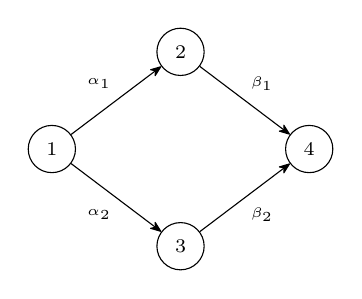
\begin{tikzpicture}[->,>={Stealth[round]},node distance=8mm and 12mm,
  every node/.style={circle,draw,minimum size=6mm,inner sep=0pt,font=\scriptsize}]
  \node (1) {1};
  \node (2) [above right=of 1] {2};
  \node (3) [below right=of 1] {3};
  \node (4) [below right=of 2] {4};
  \draw (1) -- node[draw=none,fill=none,above left,font=\tiny]{$\alpha_1$} (2);
  \draw (1) -- node[draw=none,fill=none,below left,font=\tiny]{$\alpha_2$} (3);
  \draw (2) -- node[draw=none,fill=none,above right,font=\tiny]{$\beta_1$} (4);
  \draw (3) -- node[draw=none,fill=none,below right,font=\tiny]{$\beta_2$} (4);
\end{tikzpicture}
\caption{The diamond quiver of Example~\ref{ex:diamond}: two parallel
length-$2$ walks $1\walk4$; $\dim(e_4\kQ_2 e_1)=2$.}
\label{fig:diamond}
\end{figure}

% ---------------------------------------------------------------------
\subsection{Impact degree and the fundamental neighbourhood system}
\label{sec:sfv}
% ---------------------------------------------------------------------

The grading by length induces a canonical stratification of the vertices around
each node, which organises the multi-hop structure the model will exploit. The
\emph{impact degree} $g(i,j)$ is the length of the shortest directed path from
$i$ to $j$ (with $g(i,i)=0$ and $g(i,j)=\infty$ if no directed path exists);
equivalently, $g(i,j)=\min\{k:(\Adj^{\,k})_{ij}>0\}$, the first range at which
the walk multiplicity becomes positive.

\begin{definition}\label{def:sfv}
For a node $c\in Q_0$, its \emph{in-neighbourhood} of radius $k$ is
$A_k(c)=\{i\in Q_0: g(i,c)\le k\}$, the set of nodes that can influence $c$
along a directed path of length at most $k$. The nested family
$\{A_k(c)\}_{k\ge0}$, with $A_0(c)=\{c\}\subseteq A_1(c)\subseteq\cdots$, is
the \emph{fundamental neighbourhood system} (FNS) of $c$; the layer
$\mathcal{N}_k(c)=A_k(c)\setminus A_{k-1}(c)$ collects the nodes at impact
degree exactly $k$.
\end{definition}

The FNS is the combinatorial object that the walk operators below act on, and
its precise relation to walk-reachability is the following.

\begin{proposition}\label{prop:fns}
For $k\ge1$ let $\mathcal{S}_k=\{(c,i):(\Adj^{\,k})_{ic}>0\}$ be the pairs
joined by a length-$k$ walk $i\walk c$. Then
\[
  \{(c,i): i\in \mathcal{N}_k(c)\} \;\subseteq\; \mathcal{S}_k ,
\]
and the inclusion is strict in general: length-$k$ walks may also reach nodes
at impact degree $<k$. If $Q$ is \emph{graded}---there is
$\rho\colon Q_0\to\mathbb{Z}$ with $\rho(t(\alpha))=\rho(s(\alpha))+1$ for
every arrow $\alpha$---equality holds for every $k$.
\end{proposition}

\begin{proof}
If $g(i,c)=k$, a shortest path is a length-$k$ walk, so $(\Adj^{\,k})_{ic}>0$.
Strictness: in $1\to2\to3$ with an extra arrow $1\to3$, $(\Adj^2)_{13}>0$ yet
$g(1,3)=1$. If $Q$ is graded, every walk $i\walk c$ has length
$\rho(c)-\rho(i)$, so a length-$k$ walk forces $g(i,c)=k$. \qed
\end{proof}

The benchmark graphs of Section~\ref{sec:exp} are graded (the layer index is
such a $\rho$), so there the supports coincide with the FNS layers; on graphs
with cycles, such as a ring, $\mathcal{S}_k$ strictly contains the layer
relation. Stacking ranges $k=1,2,\dots$ thus walks an embedding outward through
the layers of the FNS, and the multiplicity $n_k(i,c)$ records \emph{how many}
length-$k$ paths populate each layer---the textured, algebraic refinement of
the scalar impact degree.

% ---------------------------------------------------------------------
\subsection{Walk operators}
% ---------------------------------------------------------------------

Proposition~\ref{prop:count} lets us turn the graded path algebra into a family
of linear operators on node features, one per range; these are the bridge to
the neural model.

\begin{definition}\label{def:walkop}
For each range $k\ge1$ define $W^{(k)}\in\RR^{n\times n}$ by
\[
  W^{(k)}_{j i}\;=\;\frac{(\Adj^{\,k})_{ij}}{\,Z_k\,},
  \qquad Z_k=\max_{j}\sum_i (\Adj^{\,k})_{ij},
\]
a single normalising constant per range. The \emph{walk-reachability support}
at range $k$ is $\mathcal{S}_k=\{(j,i):(\Adj^{\,k})_{ij}>0\}$.
\end{definition}

Acting on a feature matrix $H\in\RR^{n\times d}$, the operator $W^{(k)}H$ sends
to each node $j$ a weighted sum of the features of every node $i$ that reaches
$j$ by a length-$k$ walk, the weight proportional to the multiplicity
$n_k(i,j)$. Two facts are worth stressing. \emph{(i) Global, not row,
normalisation}: row normalisation would map the multiplicities to a uniform
distribution over the reachable sources, erasing exactly the information that
distinguishes $W^{(k)}$ from a plain reachability mask; the global constant
keeps the relative multiplicities intact while bounding magnitudes.
\emph{(ii) Sparsity}: $\mathcal{S}_k$ is the nonzero pattern of $\Adj^{\,k}$,
so on the structured graphs of interest $W^{(k)}$ is stored and applied in
$O(|\mathcal{S}_k|)$ rather than $O(n^2)$. The fixed-weight $W^{(k)}$ already
mitigates over-squashing, because it lets node $j$ read from range-$k$ sources
\emph{directly}, in one step, instead of forcing the signal through $k$ rounds
of local message passing. Its limitation---which motivates Walk Attention---is
that the weights are fixed by multiplicity and cannot \emph{select} which
reachable source matters.

% ---------------------------------------------------------------------
\subsection{The quotient algebra}
% ---------------------------------------------------------------------

Representation theory routinely passes from $\kQ$ to a quotient $\kQ/I$ by an
\emph{admissible ideal} $I$, identifying paths that are declared equal. In the
diamond of Example~\ref{ex:diamond}, the relation
$\beta_1\alpha_1\equiv\beta_2\alpha_2$ generates an ideal for which
$\dim\bigl(e_4(\kQ/I)_2e_1\bigr)=1$: the two parallel walks collapse to a
single class, and in general
$\dim\bigl(e_j(\kQ/I)_ke_i\bigr)\le n_k(i,j)$. It is tempting to use this
quotient directly as an over-squashing remedy: replace the walk multiplicities
by the smaller quotient dimensions, ``de-duplicating'' redundant paths before
aggregation. We tested this and found it \emph{counterproductive}
(Section~\ref{sec:exp}): collapsing parallel walks destroys multiplicity
information that downstream tasks may require. The constructive role of the
quotient is not to compress the signal but to \emph{reshape the support}---for
instance routing distinct path classes to distinct attention heads, a direction
we leave to future work. In the model that follows the algebra enters only
through the support $\mathcal{S}_k$ and the unquotiented operators $W^{(k)}$.

% ---------------------------------------------------------------------
\subsection{A common algebraic ground}\label{sec:ground}
% ---------------------------------------------------------------------

The objects above---the graded algebra $\kQ$, the impact degree with its FNS,
and the quotient $\kQ/I$---form one algebraic substrate that specialises in two
directions, according to how a node-update map $\varphi$ over the layers
$\mathcal{N}_k(c)$ is read. In the \emph{dynamical} reading, $\varphi$ is a
fixed evolution rule weighted by impact degree; iterating it in time yields the
\emph{automata of impact over quivers} (AIQ), with its SI/SIS/SIR rules and
category structure, developed separately
\cite{zainea2026aiq,ibanez2025casimulations}. In the \emph{representational}
reading, taken here, $\varphi$ is \emph{learned}: a vector space at each vertex
and a linear map at each arrow is a representation of $Q$ (a $\kQ$-module, via
$\mathrm{Rep}(Q)\cong\kQ\text{-}\mathrm{Mod}$), and a graph neural network on
$Q$ is such a representation with learned arrow maps. Walk Attention is its
graded instance; the two readings share the trunk and differ only in whether
$\varphi$ is prescribed or learned.

% =====================================================================
\section{Walk Attention}\label{sec:model}
% =====================================================================

We now define the architecture, and we begin with the observation that
motivates it: \emph{the walk operator already is an attention}. An attention
layer, in its general form, fixes a \emph{support} relation $S$ of (target,
source) pairs and computes, for each target $j$, a normalised weighted
combination of transformed source features,
\begin{equation}\label{eq:attn-generic}
  \mathrm{out}_j \;=\; \sum_{i:\,(j,i)\in S}\alpha_{ji}\,Vx_i,
  \qquad \alpha_{ji}\ge0,\quad \textstyle\sum_{i}\alpha_{ji}\;\text{bounded},
\end{equation}
and architectures differ only in two choices: \emph{which pairs} $S$ contains,
and \emph{where the coefficients} $\alpha$ come from. Transformer
self-attention \cite{vaswani2017attention} takes $S=$ all pairs and learns
$\alpha$ from query--key products; GAT \cite{velickovic2017graph} takes $S=$
the edges and learns $\alpha$. Now compare with the walk operator of
Definition~\ref{def:walkop}: acting on features it computes
$(W^{(k)}H)_j=\sum_{i:(j,i)\in\mathcal{S}_k}\tfrac{n_k(i,j)}{Z_k}\,H_i$---
\emph{exactly the form}~\eqref{eq:attn-generic}, with support the
walk-reachability $\mathcal{S}_k$ and coefficients fixed at the normalised walk
multiplicities. Aggregating over length-$k$ walks is therefore not ``like''
attention; it \emph{is} an attention whose support the path algebra determines
exactly (Proposition~\ref{prop:count}) and whose weights happen to be frozen.
This dictates the design: keep the algebraic support and replace the frozen
multiplicity weights by learned query--key weights---the result is Walk
Attention, the learned node update $\varphi$ of the common substrate of
Section~\ref{sec:ground}.

% ---------------------------------------------------------------------
\subsection{The Walk Attention layer}\label{sec:layer}
% ---------------------------------------------------------------------

Fix a range $k$ with support $\mathcal{S}_k$. A Walk Attention layer with $H$
heads of dimension $C$ computes queries, keys and values by linear maps,
$Q^h=xW^h_Q$, $K^h=xW^h_K$, $V^h=xW^h_V$, and attends \emph{only over the
reachable pairs} $(j,i)\in\mathcal{S}_k$:
\begin{equation}\label{eq:wa}
  \ell^h_{ji} = \tfrac{1}{\sqrt{C}}\langle Q^h_j,K^h_i\rangle,\qquad
  \alpha^h_{ji} = \softmax_{i:(j,i)\in\mathcal{S}_k}\ell^h_{ji},\qquad
  z^h_j = \textstyle\sum_{i:(j,i)\in\mathcal{S}_k}\alpha^h_{ji}V^h_i.
\end{equation}
The softmax is taken, for each target $j$, over exactly the sources that reach
$j$ by a length-$k$ walk---a \emph{segmented} softmax over the support, never
over all $n$ nodes. The head outputs are concatenated and a residual ``root''
term is added, $\mathrm{WA}_k(x)_j=\Vert_h z^h_j + x_jW_{\!\text{root}}$.
Because~\eqref{eq:wa} only ever touches pairs in $\mathcal{S}_k$, the layer
costs $O(|\mathcal{S}_k|HC)$ time and memory, not $O(n^2)$; the supports are
precomputed once per graph as the nonzero patterns of $\Adj^{\,k}$.
Figure~\ref{fig:layer} shows the data flow and Algorithm~\ref{alg:wa}
summarises one layer.

\begin{figure}[t]
\centering
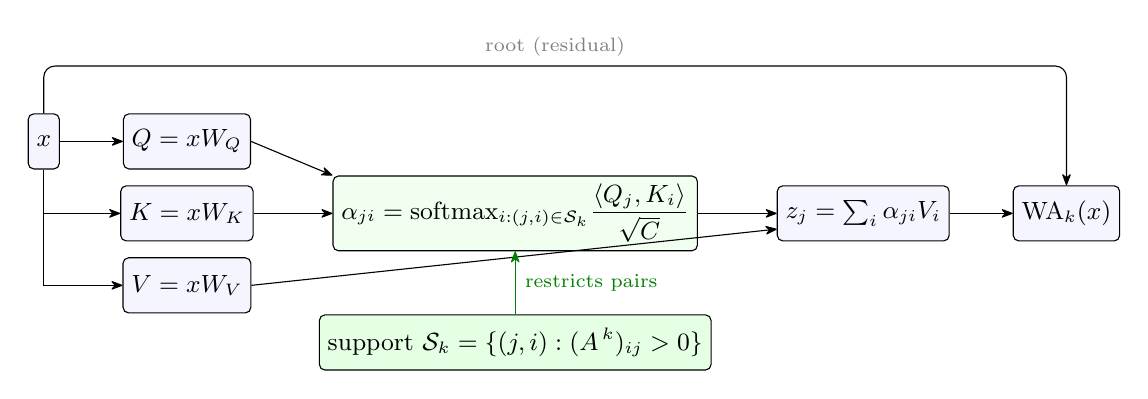
\begin{tikzpicture}[
  >={Stealth[round]}, node distance=6mm,
  box/.style={draw,rounded corners=2pt,minimum height=7mm,inner sep=3pt,font=\small,fill=blue!4},
  alg/.style={draw,rounded corners=2pt,minimum height=7mm,inner sep=3pt,font=\small,fill=green!6},
  lbl/.style={font=\scriptsize,gray}]
  \node[box] (x) {$x$};
  \node[box,right=8mm of x] (q) {$Q=xW_Q$};
  \node[box,below=2mm of q] (k) {$K=xW_K$};
  \node[box,below=2mm of k] (v) {$V=xW_V$};
  \node[alg,right=10mm of k] (att)
    {$\displaystyle \alpha_{ji}=\softmax_{i:(j,i)\in\mathcal{S}_k}\!\frac{\langle Q_j,K_i\rangle}{\sqrt C}$};
  \node[box,right=10mm of att] (agg) {$z_j=\sum_i \alpha_{ji}V_i$};
  \node[box,right=8mm of agg] (out) {$\mathrm{WA}_k(x)$};
  \node[alg,below=8mm of att,fill=green!10] (supp)
    {support $\mathcal{S}_k=\{(j,i):(\Adj^{\,k})_{ij}>0\}$};
  \draw[->] (x) -- (q.west);
  \draw[->] (x) |- (k.west);
  \draw[->] (x) |- (v.west);
  \draw[->] (q.east) -- (att.north west);
  \draw[->] (k.east) -- (att.west);
  \draw[->] (att.east) -- (agg.west);
  \draw[->] (v.east) -- ([yshift=-2mm]agg.west);
  \draw[->] (agg) -- (out);
  \draw[->,green!50!black] (supp.north) -- (att.south)
    node[midway,right,lbl,text=green!50!black] {restricts pairs};
  \draw[->,rounded corners] (x.north) -- ++(0,6mm) -| (out.north)
    node[pos=0.25,above,lbl] {root (residual)};
\end{tikzpicture}
\caption{One Walk Attention layer at range $k$. Queries, keys and values are
linear maps of the node features; attention is computed \emph{only} over the
walk-reachable pairs $\mathcal{S}_k$ supplied by the path algebra (the nonzero
pattern of $\Adj^{\,k}$), then aggregated and added to a residual root term.
The green support box is what distinguishes Walk Attention from dense
($\mathcal{S}_k=$ all pairs) and one-hop ($\mathcal{S}_k=$ edges) attention.}
\label{fig:layer}
\end{figure}

\begin{example}\label{ex:layer}
In the diamond of Example~\ref{ex:diamond} at range $k=2$ the support is the
single pair $\mathcal{S}_2=\{(4,1)\}$: node $4$ attends directly to node $1$,
the softmax over a singleton gives $\alpha_{41}=1$, and
$\mathrm{WA}_2(x)_4=Vx_1+x_4W_{\!\text{root}}$---the two parallel walks become
one \emph{direct} interaction. Adding a second source $1'$ with arrows to $2$
and $3$ gives $\mathcal{S}_2=\{(4,1),(4,1')\}$: the softmax now weighs the two
sources by the match of their keys against the query $Qx_4$, so node $4$ reads
both range-$2$ sources directly \emph{and chooses between them}---whereas a
one-hop network must push both signals through the shared vertices $2,3$, the
very compression that over-squashing names.
\end{example}

A depth-$L$ Walk Attention network stacks one layer per range $k=1,\dots,L$, so
successive layers read from progressively longer walks; each layer is followed
by layer normalisation, an \textsc{elu} nonlinearity and dropout, and a final
MLP maps the embedding to task outputs. Layer normalisation is important in
practice: without it the learned attention is high-variance across
initialisations; with it, together with a short learning-rate warmup and
gradient clipping, training converges reliably (Section~\ref{sec:exp}).

\begin{algorithm}[t]
\caption{Walk Attention layer at range $k$ (sparse).}\label{alg:wa}
\begin{algorithmic}[1]
\Require features $x\in\RR^{n\times d_{\text{in}}}$; support
  $\mathcal{S}_k=\{(j,i):(\Adj^{\,k})_{ij}>0\}$
\State $Q,K,V \gets xW_Q,\,xW_K,\,xW_V$ \Comment{per head; shapes $n\times HC$}
\For{each $(j,i)\in\mathcal{S}_k$ and head $h$}
  \State $\ell^h_{ji}\gets \langle Q^h_j,K^h_i\rangle/\sqrt{C}$
\EndFor
\State $\alpha^h_{ji}\gets$ segmented-$\softmax$ over $\{i:(j,i)\in\mathcal{S}_k\}$
\State $z^h_j\gets \sum_i \alpha^h_{ji}V^h_i$ \Comment{scatter-add into targets}
\State \Return $\bigl\Vert_h z^h \;+\; xW_{\!\text{root}}$
\end{algorithmic}
\end{algorithm}

Table~\ref{tab:relation} situates Walk Attention among related operators along
the two axes of~\eqref{eq:attn-generic}. A one-hop GAT layer learns weights but
must propagate long-range signal through $L$ stacked layers---precisely the
over-squashing regime; a full graph Transformer learns weights over all pairs,
paying $O(n^2)$ and discarding structure unless positional encodings reinject
it; the walk operator has the right multi-hop support but cannot select. Walk
Attention occupies the remaining cell: multi-hop, structure-aware support
\emph{and} learned, selective weights.

\begin{table}[t]
\centering
\caption{Walk Attention against related aggregation operators, by the two axes
of~\eqref{eq:attn-generic}: support and weights.}
\label{tab:relation}
\begin{tabular}{lccc}
\toprule
\textbf{Operator} & \textbf{Support} & \textbf{Weights} & \textbf{Cost} \\
\midrule
GCN / message passing       & 1-hop      & fixed (degree) & $O(|Q_1|)$ \\
Graph attention (GAT)       & 1-hop      & learned        & $O(|Q_1|)$ \\
Walk operator $W^{(k)}$     & walk-reachable & fixed (multiplicity) & $O(|\mathcal{S}_k|)$ \\
Graph Transformer           & all pairs  & learned        & $O(n^2)$ \\
\textbf{Walk Attention (ours)} & \textbf{walk-reachable} & \textbf{learned} & $O(|\mathcal{S}_k|)$ \\
\bottomrule
\end{tabular}
\end{table}

% ---------------------------------------------------------------------
\subsection{A formal account on the bottleneck family}\label{sec:theory}
% ---------------------------------------------------------------------

On the bottleneck-chain family used in Section~\ref{sec:exp}, the separation
between one-hop message passing and Walk Attention can be \emph{proved}, not
only measured. The construction: $K$ sources carry a one-hot \emph{key}---the
key assignment is a uniformly random permutation $\pi$---and a one-hot
\emph{value}; $d$ bottleneck layers $L_1,\dots,L_d$ of $M$ interchangeable,
featureless vertices follow, consecutive layers fully connected; a target
carries a one-hot \emph{query} $q$ and must output the value of the source
whose key is $q$ (label $\pi^{-1}(q)$, chance $1/K$). Networks have the
standard depth $L=d+1$---one layer per hop, as in \cite{alon2021bottleneck} and
in our experiments---and hidden width $w$.

\begin{proposition}\label{prop:collapse}
For any message-passing network whose update
$h_v'=U\bigl(h_v,\mathrm{AGG}\{h_u:u\to v\}\bigr)$ is shared across vertices:
after every round, all $M$ vertices of each bottleneck layer carry identical
states. Hence the entire influence of the sources on the target passes through
a single $w$-dimensional state per layer---while $K M^{d}$ walks carry it
(Proposition~\ref{prop:count}).
\end{proposition}

\begin{proof}
Induction on the round: vertices of a layer start equal (zero features) and
share their in-multiset (all sources for $L_1$, all of $L_{r-1}$ for $L_r$), so
shared $U,\mathrm{AGG}$ keep them equal. \qed
\end{proof}

\begin{proposition}\label{prop:blind}
If moreover messages are linear in the sender's state with content-independent
coefficients---as in GCN and GIN---then with $L=d+1$ layers the target's output
depends on the sources only through $\sum_s x_s$, which is the same for every
$\pi$: the one-hot keys of a permutation sum to the all-ones vector. Expected
accuracy is exactly $1/K$ for every $d$, $w$, and parameters.
\end{proposition}

\begin{proof}
Source information entering $L_1$ at round $t$ needs $d$ more hops, reaching
the target at round $t+d\le d+1$ only if $t\le1$; at round $1$ the message from
source $s$ is a fixed linear map of the raw $x_s$ with one shared coefficient
(sources are isomorphic in the graph), so $L_1$'s state is a function of
$\sum_s x_s$, whose key and value blocks are $\pi$-independent. Given $q$, the
label $\pi^{-1}(q)$ is uniform, so a $\pi$-independent prediction scores $1/K$.
\qed
\end{proof}

\begin{proposition}\label{prop:wa}
At range $k=d+1$ the target's support is exactly the $K$ sources (the graph is
graded; Proposition~\ref{prop:fns}). With $W_Q$ projecting the query slot
scaled by any $\beta>0$, $W_K$ the key slot, $W_V$ the value slot and
$W_{\!\text{root}}=0$, the output $z_t=\sum_s\alpha_s e_{v(s)}$ of a single
Walk Attention layer has its largest entry at the correct value, on every
instance, for all $d$ and $M$.
\end{proposition}

\begin{proof}
The logit of source $s$ is $\beta\,\mathbf{1}[\pi(s)=q]$, so the softmax puts
its largest weight $e^{\beta}/(e^{\beta}+K-1)$ on the unique match $s^\ast$;
the values being distinct basis vectors, the largest coordinate of $z_t$ is
$\alpha_{s^\ast}$, at $v(s^\ast)=\pi^{-1}(q)$. \qed
\end{proof}

\begin{example}\label{ex:blind}
Take $K=2$, $M=2$, $d=1$ and depth $L=2$. The two key assignments,
$\pi=\mathrm{id}$ and the swap, produce the \emph{same} source sum
$\sum_s x_s$ (key and value blocks both $(1,1)$), so by
Proposition~\ref{prop:blind} a GCN or GIN computes identical outputs on the two
instances---whose labels differ: accuracy $1/2$, chance. A Walk Attention layer
at range $2$ attends over $\{s_1,s_2\}$ with logits
$\beta\langle e_q,e_{\pi(s)}\rangle$, which distinguish the instances at the
first multiplication and select the matching source
(Proposition~\ref{prop:wa}).
\end{example}

\begin{remark}\label{rem:mechanisms}
The propositions delimit the mechanisms seen in Section~\ref{sec:exp}. GAT
escapes Proposition~\ref{prop:blind}---its first-round coefficients depend on
source content---but must still thread the key--value association through the
single-vector channel of Proposition~\ref{prop:collapse}, re-encoded $d+1$
times: empirically it sits above chance and degrades with depth. The
fixed-weight walk operator reads the sources directly but with \emph{equal}
weights (all multiplicities are $M^d$), so it must embed the whole key--value
multiset in $w$ dimensions rather than select one source: it plateaus in
between. Walk Attention both reads directly and selects
(Proposition~\ref{prop:wa}), and solves the task.
\end{remark}

% =====================================================================
\section{Experiments}\label{sec:exp}
% =====================================================================

We evaluate on a controlled family in which over-squashing is severe and
tunable, then on two external benchmarks. All code, configurations and
experiment logs are released \cite{repo_walkattention}.

\paragraph{Bottleneck-chain retrieval.}
We instantiate the family of Section~\ref{sec:theory} with $K{=}5$, $M{=}4$ and
depths $d\in\{2,3\}$: the walk multiplicity into the target is $KM^d$
(Proposition~\ref{prop:count}), while the deepest support consists of only the
$K$ source--target pairs ($5/196\approx2.6\%$ of node pairs at $d{=}2$,
$5/324\approx1.5\%$ at $d{=}3$). All models use hidden width $16$, four heads
where applicable, $d{+}1$ layers/ranges, and AdamW with a ten-epoch warmup,
cosine decay and gradient clipping; Walk Attention adds layer normalisation. We
report validation target accuracy (the synthetic task has no separate test
split), mean $\pm$ std over five seeds. Table~\ref{tab:main} lands exactly
where Propositions~\ref{prop:collapse}--\ref{prop:wa} put it
(Remark~\ref{rem:mechanisms}): GCN and GIN are pinned at chance and sit there
empirically; GAT degrades sharply with depth; the walk operator crosses the
bottleneck in one step but, weighting all sources by multiplicity alone,
cannot select the matching one and plateaus; \textbf{Walk Attention solves the
task exactly} at both depths over all seeds. Without layer normalisation and
warmup its accuracy ranged $0.44$--$1.00$ across seeds; the three standard
stabilisers remove this variance entirely---an optimisation artefact, not a
property of the operator.

\begin{table}[t]
\centering
\caption{Target accuracy (mean $\pm$ std over 5 seeds) on bottleneck-chain
retrieval, $K{=}5$, $M{=}4$; chance $1/K=0.20$; the answer lies $d{+}1$ hops
away. GCN/GIN sit at chance as Proposition~\ref{prop:blind} mandates (the
residual $+0.01$--$0.02$ is best-epoch selection on a finite validation
split).}
\label{tab:main}
\begin{tabular}{lcc}
\toprule
\textbf{Model} & \textbf{depth $d=2$} & \textbf{depth $d=3$} \\
\midrule
GCN (one-hop, linear aggregation)  & $0.21\pm0.01$ & $0.22\pm0.01$ \\
GIN (one-hop, linear aggregation)  & $0.21\pm0.01$ & $0.21\pm0.01$ \\
GAT (one-hop attention)            & $0.45\pm0.22$ & $0.29\pm0.17$ \\
Walk operator (fixed weights)      & $0.62\pm0.12$ & $0.50\pm0.12$ \\
\textbf{Walk Attention (ours)}     & $\mathbf{1.000\pm0.000}$ & $\mathbf{1.000\pm0.000}$ \\
\bottomrule
\end{tabular}
\end{table}

\paragraph{RingTransfer.}
The bottleneck family is our own construction; to confirm the effect on an
independent benchmark we use \textsc{RingTransfer}
\cite{digiovanni2023oversquashing}: a cycle of $n$ nodes in which a source must
transmit its one-hot label (five classes, chance $0.2$) to the diametrically
opposite target, $n/2$ hops away along the \emph{two arcs} of the ring. Every
node has two neighbours, so the number of length-$(n/2)$ walks entering the
target---what a one-hop network must compress after $n/2$ layers---grows as
$2^{n/2}$, while only the two arc walks carry the signal. All models use hidden
width $32$, the same optimiser recipe, and $n/2$ layers/ranges.
Table~\ref{tab:ring} reports the results: small rings are easy for every model;
from $n{=}14$ (distance $7$) the one-hop baselines degrade and become highly
seed-dependent---at $n{=}18$ GAT falls to $0.29\pm0.19$ and GCN to
$0.53\pm0.33$---while \textbf{Walk Attention stays at $1.000\pm0.000$
throughout}. The gap widens with ring size, i.e.\ with the severity of
over-squashing, as predicted.

\begin{table}[t]
\centering
\caption{\textsc{RingTransfer} accuracy vs.\ ring size $n$ (distance $n/2$),
mean $\pm$ std over 5 seeds; chance $0.20$.}
\label{tab:ring}
\begin{tabular}{lcccc}
\toprule
\textbf{Model} & $n{=}6$ & $n{=}10$ & $n{=}14$ & $n{=}18$ \\
\midrule
GCN                    & $1.00\pm0.00$ & $1.00\pm0.00$ & $0.81\pm0.13$ & $0.53\pm0.33$ \\
GAT                    & $1.00\pm0.00$ & $1.00\pm0.00$ & $0.69\pm0.29$ & $0.29\pm0.19$ \\
\textbf{Walk Attention (ours)} & $\mathbf{1.00\pm0.00}$ & $\mathbf{1.00\pm0.00}$ & $\mathbf{1.00\pm0.00}$ & $\mathbf{1.00\pm0.00}$ \\
\bottomrule
\end{tabular}
\end{table}

\paragraph{Collapsing walks hurts.}
The quotient $\kQ/I$ of Section~\ref{sec:algebra} suggests an alternative
remedy: replace the multiplicities $n_k(i,j)$ by the smaller quotient
dimensions, de-duplicating equivalent walks before aggregation. We compare the
quotient-built fixed-weight operator to the raw one in an ablation that changes
\emph{only} the operator and holds everything else---data, architecture, and
the optimiser recipe of Table~\ref{tab:main}---fixed. Table~\ref{tab:quotient}
shows the quotient falling clearly below the raw operator at both depths:
collapsing parallel walks discards the source multiplicity that the retrieval
task needs. In this regime redundant paths are \emph{signal}, not noise; the
algebra's contribution is the support, not compression. Whether a regime exists
where the quotient's compression helps---genuinely redundant parallel paths, or
path classes routed to distinct heads---remains open.

\begin{table}[t]
\centering
\caption{De-duplicating walks via $\kQ/I$ \emph{hurts}: mean $\pm$ std over 5
seeds, same protocol as Table~\ref{tab:main} (the walk-operator row coincides).}
\label{tab:quotient}
\begin{tabular}{lcc}
\toprule
\textbf{Operator} & \textbf{depth $d=2$} & \textbf{depth $d=3$} \\
\midrule
Quotient $\kQ/I$ (collapsed walks) & $0.39\pm0.04$ & $0.30\pm0.09$ \\
Walk operator (raw walks)          & $\mathbf{0.62\pm0.12}$ & $\mathbf{0.50\pm0.12}$ \\
\bottomrule
\end{tabular}
\end{table}

\paragraph{LRGB Peptides-func.}
The synthetic benchmarks are deliberately worst cases; to assess real data we
use Peptides-func \cite{dwivedi2022lrgb} ($10{,}873/2{,}331/2{,}331$ molecular
graphs, median $138$ nodes; multi-label classification, test Average
Precision), with the same atom embedding, four layers, hidden width $80$, mean
pooling and AdamW for every model; Walk Attention uses ranges $k=1,\dots,4$,
whose support stays sparse ($1$--$8\%$ of $n^2$ at range $3$).
Table~\ref{tab:lrgb}: Walk Attention exceeds GCN and is statistically
indistinguishable from GAT ($0.526\pm0.007$ vs.\ $0.526\pm0.004$ over four
seeds). Two caveats frame the comparison. First, all models share a
deliberately small budget, so absolute numbers sit below published results
(GCN $0.593$ under the tuned $500$k-parameter protocol \cite{dwivedi2022lrgb},
higher still in re-evaluations \cite{tonshoff2023where}): the comparison is
\emph{internal}, isolating the aggregation operator. Second, the tie is not for
lack of parallel paths (peptides contain hundreds of vertex pairs joined by
several short walks) but because over-squashing is \emph{mild} on these small
graphs. The advantage of the multi-hop support is therefore
\emph{regime-dependent}: decisive when squashing is severe
(Tables~\ref{tab:main}--\ref{tab:ring}), modest when it is mild, at about
$1.6\times$ GAT's wall-clock---far below dense all-pairs attention.

\begin{table}[t]
\centering
\caption{LRGB Peptides-func, test AP (mean $\pm$ std over 4 seeds), shared
small budget isolating the operator; published results under the standard
$500$k protocol are higher for every architecture
\cite{dwivedi2022lrgb,tonshoff2023where}.}
\label{tab:lrgb}
\begin{tabular}{lc}
\toprule
\textbf{Model} & \textbf{test AP} \\
\midrule
GCN                          & $0.492\pm0.011$ \\
GAT                          & $0.526\pm0.004$ \\
Walk Attention (ours)        & $0.526\pm0.007$ \\
\bottomrule
\end{tabular}
\end{table}

% =====================================================================
\section{Conclusion and Future Work}\label{sec:conclusion}
% =====================================================================

We introduced Walk Attention, an architecture that mitigates over-squashing by
attending over a multi-hop support supplied by the path algebra of the
underlying quiver. Proposition~\ref{prop:count} gives the support and its
multiplicities exactly; Propositions~\ref{prop:collapse}--\ref{prop:wa} prove
the separation on the bottleneck family---message passing with linear first
aggregation is at chance for every depth and width, while one Walk Attention
layer at the matching range is exact---and the experiments confirm it, with a
regime-dependent advantage on \textsc{RingTransfer} and Peptides-func. A
complementary negative result showed that compressing equivalent walks via the
quotient is counterproductive when multiplicity carries signal: the role of the
algebra is to determine the attention support, not to discard information. The
construction is deliberately elementary and self-contained, an entry point
connecting quiver representation theory to graph representation learning; it
is the learned reading of a common substrate whose dynamical reading is the
AIQ framework \cite{zainea2026aiq}. Several directions follow.

\begin{itemize}
  \item \textbf{From learned weights to dynamics.} Inject the attention weights
  learned on a task into an AIQ as a data-driven evolution rule, reading off
  the dynamical effect of each weight, and conversely let AIQ stability and
  reachability analyses interpret and constrain what Walk Attention has
  learned---to us the most promising bridge.
  \item \textbf{Benchmarks with severe over-squashing.} Real long-range tasks
  whose graphs contain acute bottlenecks, compared against rewiring
  \cite{topping2022understanding}, multi-hop \cite{gutteridge2023drew} and
  graph-Transformer baselines.
  \item \textbf{Quotient-shaped supports.} Use $\kQ/I$ to \emph{partition}
  walks into equivalence classes routed to distinct attention heads, rather
  than to compress; identifying which relations $I$ are useful, and learning
  them from data, is an appealing problem.
  \item \textbf{Scaling the support.} Truncate, sample, or learn sparser
  admissible supports on dense graphs, where the range-$k$ support can itself
  grow large.
\end{itemize}

\subsubsection*{Reproducibility.}
All graph generators, the walk operators, the Walk Attention layer, the
baselines and the experiment logs are released \cite{repo_walkattention}; the
path-algebra computations build on the open-source \texttt{aiq-quivers} library
\cite{repo_aiqquivers}.

% =====================================================================
\bibliographystyle{splncs04}
\bibliography{walk_attention}
% =====================================================================

\end{document}
